\documentclass[conference]{IEEEtran}

\usepackage[dvips]{graphicx}
\usepackage{amsmath,amssymb}
\usepackage{amsfonts}
%\usepackage{algorithmic,algorithm}
%\usepackage{multirow}
%\usepackage{hhline}
\usepackage{url}
\usepackage{xcolor}
\usepackage{balance}
%\usepackage{flushend}
%\usepackage{booktabs}
%\usepackage{siunitx}
\usepackage{comment}



\newcommand{\TODOnote}[1]{{\bf\color{red} TODO: #1}}
\newcommand*{\etal}{{\it et al.}}




\begin{document}

\title{	Keyboard auto-correction plugin}
\date{}%date stay empty

\author{
\IEEEauthorblockN{%
Daria Gorbunova, Vsevolod Averkov, Kirill Kulakov}
\IEEEauthorblockA{%
Petrozavodsk State University (PetrSU)\\ 
Petrozavodsk, Russia\\
\ \{gorbunov, averkov, kulakov\}@cs.petrsu.ru\\}}
\maketitle

\begin{abstract}
 Autocorrection is a really valuable helper in modern life, especially in smartphones. Nowadays we can even write an essay with our phones and most of us use phones to text friends. It helps us to avoid most errors that appear in ours texts due to the lack of grammar knowledge or rush.
The article presents a software tool for text autocorrection. The application can correct your errors while you are texting. 
\end{abstract}

\medskip
The article presents a solution based on the analysis of the input word.
The algorithm continuously checks the tree for the closest possibly correct word to the input word and returns it to the user. Plugin was created for the Aurora mobile operating system (Sailfish OS).

There are a lot of approaches to autocorrection, but the dircitonary approach has the most amount of advantages. This method allows the smallest number of errors. Moreover, only the dictionary method allows implementing in the auto-correction program the advancement of alternatives to the word being verified and the adoption of one of them as an automatic correction, which is necessary and can be used for auto-correction for the virtual keyboard (since the post-control of automatically corrected places by the user is provided).

Determining the possible correct word is a difficult task, we can choose the closest word to the input word in the dictionary, but we should be careful to decide which algorithm to use to realize every word check because the simple sorting will take a lot of time and memory. Our solution to that problem is using trees as a structure for the dictionary. Because of them the process of spellcheck will be faster due to the 
lack of need to check every single word in most cases. The most fitting kind of trees for this task is Burkhard Keller Tree. 

It is also useful to observe the Livenstein's distance. This distance forms a metric space. And metric space is any relation that meets some basic criteria:
\begin{enumerate}
\item $D(x, y) = 0 <=> x = y $ if the distance between $x$ and $y$ is zero, then $x=y$

\item $D(x, y) = D(y, x)$ the distance from $x$ to $y$ is equal to the distance from $y$ to $x$

\item $D(x, y) + D(y, z)\geqslant D(x, z)$ 
This is called a triangle inequality. The path from $x$ to $z$ should not be longer than any path passing through another intermediate point.
\newline $D(x, y)$ - integer discrete metric. 	
\end{enumerate}


Let's say we have parameters:
$dist$ -is the resulting distance
$Str$-the string we use in our search. 
$n$ - is the maximum distance that $Str$ can be from the request and still return.
Suppose we take an arbitrary string and compare it with $Str$. Since we know that the triangle inequality holds, all our results should have the largest distance $dist$+$n$.
The overall architecture is shown in the Figure~\ref{arh}.
\begin{figure}[!hbt]
	\centering
	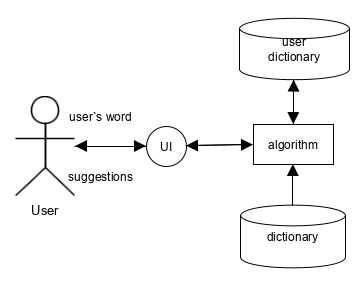
\includegraphics[width=0.3\textwidth]{images/pic.png}
	\caption{
		Arcitecture of spelling appilcstion}
	\label{arh}
\end{figure}

In the current stage of this progect four possible outcomes are possible for the user: there are no possible variant for correct word (see Fig.~\ref{zero}), there is one possible variant for correct word (see Fig.~\ref{one}) there are two possible variants for correct word (see Fig.~\ref{two}) and there are three possible variants for correct word(see Fig.~\ref{three}). 

\begin{figure}[!hbt]
	\centering
 	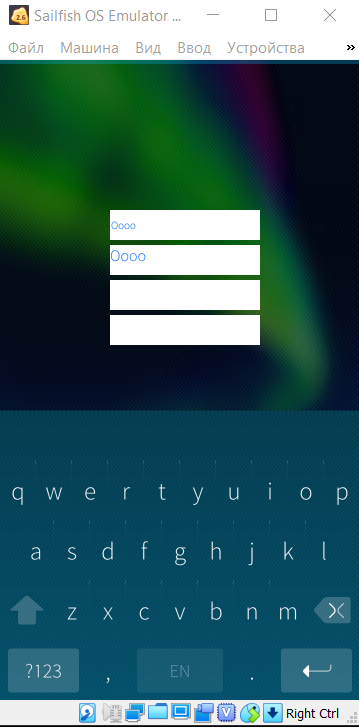
\includegraphics[width=0.3\textwidth]{images/0.png}
	\caption{No possible variant for correct word}
	\label{zero}
\end{figure}

\begin{figure}[!hbt]
	\centering
	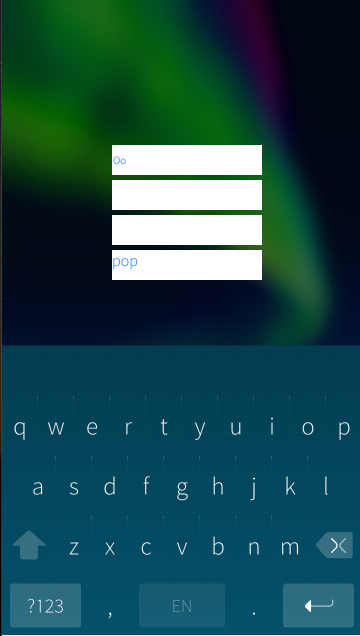
\includegraphics[width=0.3\textwidth]{images/1.png}
	\caption{One possible variant for correct word}
	\label{one}
\end{figure}


\begin{figure}[!hbt]
	\centering
	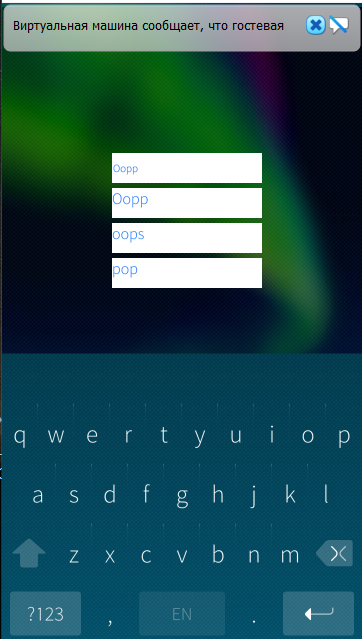
\includegraphics[width=0.3\textwidth]{images/2.png}
	\caption{Two possible variants for correct word
	}
	\label{two}
\end{figure}

\begin{figure}[!hbt]
	\centering
	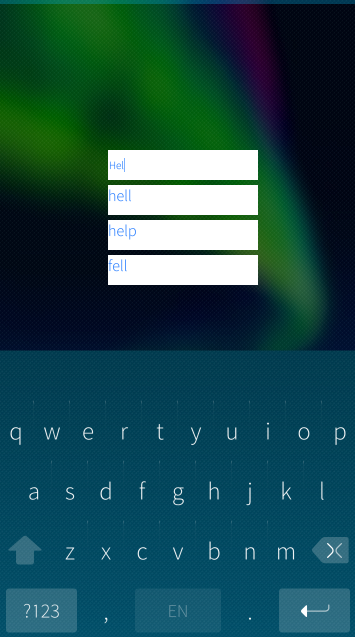
\includegraphics[width=0.3\textwidth]{images/3.png}
	\caption{
		 Three possible variants for correct word}
	\label{three}
\end{figure}
\




\begin{enumerate} 
	
	\bibitem{a} 

\end{enumerate}

\end{document}






